\documentclass[10pt,twocolumn]{article}
\usepackage[margin=0.75in,columnsep=0.28in]{geometry}
\usepackage{graphicx}
\usepackage{booktabs}
\usepackage{amsmath}
\usepackage[T1]{fontenc}
\usepackage{lmodern}
\usepackage{microtype}
\usepackage[hidelinks]{hyperref}
\usepackage{caption}
\captionsetup{font=small,labelfont=bf}
\setlength{\textfloatsep}{8pt plus 2pt minus 2pt}
\renewcommand{\topfraction}{0.9}
\renewcommand{\bottomfraction}{0.8}
\renewcommand{\textfraction}{0.1}
\renewcommand{\floatpagefraction}{0.8}
\renewcommand{\dbltopfraction}{0.9}

\title{\vspace{-1.2em}Can a Decision Model Play Figgie?\\[2pt]
\large A Small Study of Jev against Classical Card Counting}
\author{Jace\\\small\url{https://github.com/jaceyang97/figgie-on-jev}}
\date{25 September 2026}

\begin{document}
\maketitle

\begin{figure*}[t]
\centering
\begin{minipage}[b]{0.52\textwidth}\centering
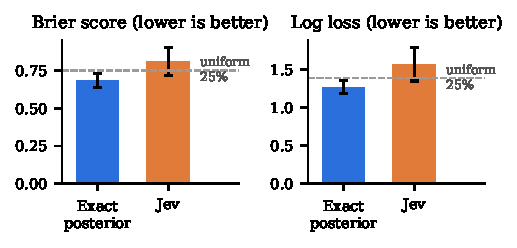
\includegraphics[width=\linewidth]{figures/compare_scores.pdf}
\caption{Goal-suit forecasts at 100 frozen states, with bootstrap 95\% CIs. The dashed line is a uniform 25\% guess.
Jev scores worse than uniform on both rules; the exact posterior scores better.}
\label{fig:scores}
\end{minipage}\hfill
\begin{minipage}[b]{0.42\textwidth}\centering
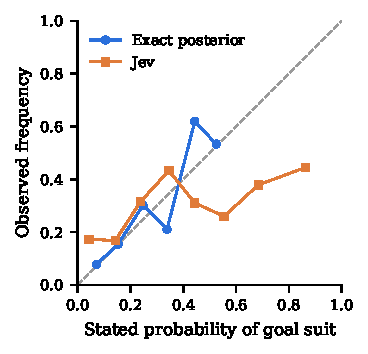
\includegraphics[width=0.8\linewidth]{figures/compare_calibration.pdf}
\caption{Reliability of the 400 suit probabilities (4 suits $\times$ 100 states), binned. When Jev says 60--90\%,
the suit is the goal suit about 30--45\% of the time.}
\label{fig:calib}
\end{minipage}
\end{figure*}


\begin{abstract}
We test TypeSafe's Jev decision model (\texttt{typesafe/jev-1.13}, via OpenRouter) as a Figgie player in a
discrete-event simulator. In the first experiment, Jev and an exact Bayesian card counter are asked about the same
100 frozen game states. Jev picks the goal suit as often as the posterior does (32\% top-1 accuracy), but it is
overconfident: its Brier score (0.81) is worse than a uniform guess (0.75), while the posterior's is better (0.69).
In the second experiment, seven prompted ``personalities'' each take one seat against the same three classical
opponents for 20 games. None earns a positive profit. The two that barely trade (\emph{timid}, \emph{value}) lose
the least; the most active ones (\emph{momentum}, \emph{hoarder}, \emph{gambler}) lose 220--250 chips a game, more
than a random noise trader. The whole study used 15{,}947 Jev calls and cost \$1.63.
\end{abstract}

\section{Setup}
\textbf{Game.} Figgie is a four-player trading game with a 40-card deck of four suits: one suit has 12 cards,
one 8, two 10. The \emph{goal suit} is the same colour as the 12-card suit. Each goal card pays 10 chips at the end
and the player with the most goal cards takes the rest of the 200-chip pot. Players start with 350 chips and ante 50,
so P\&L sums to zero over the table.

\textbf{Simulator.} One best bid and ask per suit; every trade clears all quotes. Agents wake at random times and
their orders reach the book after a latency, so slow agents lose races. Games last 240 simulated seconds.
Classical agents wake once a second with 50\,ms latency. A Jev agent wakes every two seconds on average and its
latency is the measured round trip of the API call (median 0.32\,s, 95th percentile 0.41\,s).

\textbf{Agents.} The \emph{fundamentalist} counts cards, computes the exact posterior over the 12 possible decks,
and trades against fair value. The \emph{bottom-feeder} trades against recent prices and \emph{noise} trades
randomly. A Jev agent sends a JSON description of the game (hand, chips, book, recent trades, cards known to exist)
and one Choice question listing every legal action (at most 73). A \emph{personality} is one or two sentences added
to the question's instructions. Jev is not given the posterior.

\section{Experiment 1: beliefs and actions}
In 20 games of a fundamentalist against bottom-feeder, noise and fundamentalist opponents, we froze 100 of the
fundamentalist's decision points (5 per game) and asked Jev, in one call each, which suit is the goal suit and which
action it would take.



\textbf{Beliefs.} Both forecasters name the right suit 32\% of the time, but they rarely name the same one (20\%
top-1 agreement; mean total variation distance 0.36). Jev's top probability averages 0.60 against 0.39 for the
posterior, and that confidence is not earned: its Brier score is $0.81$ [0.72, 0.91] against $0.69$ [0.64, 0.73]
for the posterior and $0.75$ for uniform, and its log loss is $1.56$ against $1.26$ and $\ln 4 = 1.39$
(Fig.~\ref{fig:scores}). Fig.~\ref{fig:calib} shows the gap is at the high end of the scale.

\textbf{Actions.} Jev chose the fundamentalist's exact action 3\% of the time. The two play different games
(Fig.~\ref{fig:actions}): the fundamentalist posts quotes at 90\% of its decisions, while Jev passes at 47\% and
never posts an offer to sell. Jev's regret against the best available take was small, 0.98 chips per decision
[0.61, 1.39], because passing and quoting cost nothing at the moment of decision.

\begin{figure}[t]
\centering
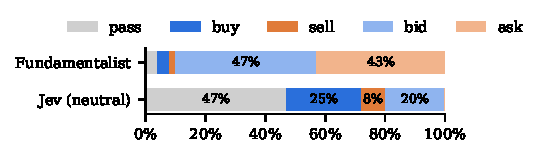
\includegraphics[width=\columnwidth]{figures/compare_actions.pdf}
\caption{Action mix at the same 100 states.}
\label{fig:actions}
\end{figure}

\section{Experiment 2: personalities}
Each personality took one seat against fundamentalist, bottom-feeder and noise for 20 games (same seed, so the same
deals), and each made about 2{,}000 Jev calls. For reference, the fundamentalist and the noise trader took the same
seat too.


\begin{figure}[t]
\centering
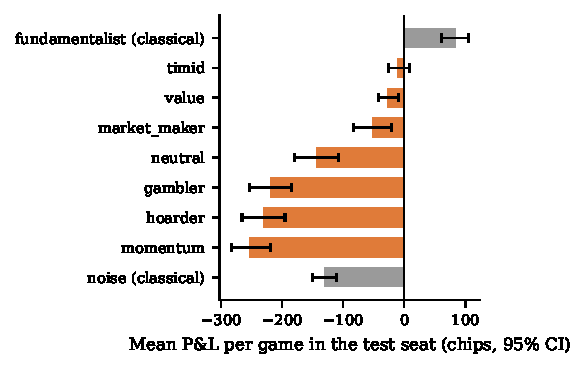
\includegraphics[width=\columnwidth]{figures/sweep_pnl.pdf}
\caption{Mean P\&L of the test seat over 20 games with bootstrap 95\% CIs. Grey bars are classical agents in the same seat.}
\label{fig:pnl}
\end{figure}

\begin{table}[t]
\centering
\small
\begin{tabular}{lrrrr}
\toprule
Seat & P\&L & Trades & Pass & Mispr. \\
\midrule
fundamentalist$^\dagger$ & $+83.4$ & 41.1 & -- & 7.13 \\
timid & $-10.7$ & 0.1 & 100\% & 6.52 \\
value & $-27.9$ & 0.5 & 99\% & 6.77 \\
market\_maker & $-51.9$ & 20.1 & 36\% & 7.22 \\
noise$^\dagger$ & $-130.4$ & 54.6 & -- & 7.15 \\
neutral & $-143.1$ & 39.6 & 43\% & 9.07 \\
gambler & $-219.4$ & 61.5 & 6\% & 9.68 \\
hoarder & $-231.0$ & 47.5 & 5\% & 9.14 \\
momentum & $-253.2$ & 47.7 & 19\% & 9.26 \\
\bottomrule
\end{tabular}
\caption{Sweep results per game. Trades are the test seat's; Pass is the share of Jev decisions that passed;
Mispr.\ is the market's mean mispricing in chips. $^\dagger$Classical agent in the test seat.}
\label{tab:sweep}
\end{table}

\textbf{Profit.} No personality made money (Fig.~\ref{fig:pnl}, Table~\ref{tab:sweep}). \emph{Timid} and
\emph{value} came closest because they almost never trade: they pass at 99--100\% of decisions, so they just hold
their dealt hand, whose expected P\&L is zero. Among personalities that did trade, \emph{market\_maker} lost least
($-52$). \emph{Momentum}, \emph{hoarder} and \emph{gambler} lost more than the random noise trader, and the loss broadly
grows with activity (Fig.~\ref{fig:tradespnl}): every extra trade was, on average, a trade against a better-informed
counterparty.

\textbf{Prompts do change behaviour.} The personalities are clearly distinguishable in what Jev chose
(Fig.~\ref{fig:mix}): \emph{hoarder} bid 60\% of the time, \emph{market\_maker} posted most of the offers to sell
(10\%, against 4\% or less for the rest), and \emph{gambler} took prices most. The instructions steer Jev strongly; they do not make it profitable.

\textbf{Effect on the market.} The \emph{neutral}, \emph{gambler}, \emph{hoarder} and \emph{momentum} seats raised mean mispricing from about 7.1 chips (classical seat) to
9.1--9.7, and the fundamentalist opponent earned most from them (up to $+200$ against \emph{momentum}).


\begin{figure}[t]
\centering
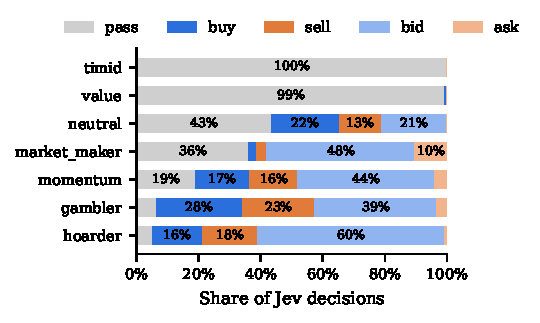
\includegraphics[width=\columnwidth]{figures/sweep_actions.pdf}
\caption{What each personality chose, over about 2{,}000 Jev decisions each.}
\label{fig:mix}
\end{figure}

\begin{figure}[t]
\centering
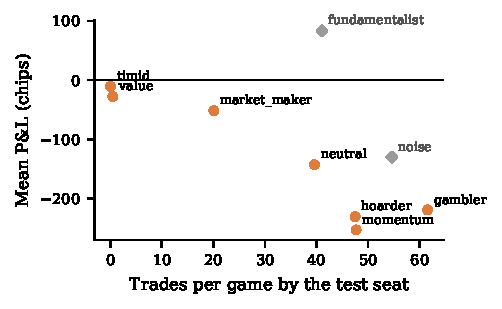
\includegraphics[width=\columnwidth]{figures/sweep_trades_pnl.pdf}
\caption{Activity against profit. Among Jev seats, more trading meant larger losses.}
\label{fig:tradespnl}
\end{figure}

\section{Discussion and limits}
Jev, used alone, reads Figgie's evidence about as accurately as exact counting on the top pick, but its
probabilities are overconfident and its trading loses to simple classical rules. The fundamentalist wins because it
turns a calibrated posterior into prices; Jev is asked to do both steps from text, and it is weakest at the numeric
one, consistent with the vendor's note that Jev is weaker with numbers.

The results are small-sample and specific to this setup: 20 games per condition, one seed, one opponent field, a
simplified market, and Jev playing at half the classical wake rate and about six times the latency. The obvious next
test is the hybrid already in the code (\texttt{jev:<personality>+assist}), where code supplies the exact posterior
and Jev only decides what to do with it.

\textbf{Reproduce.} From the repository root:
{\footnotesize
\begin{verbatim}
python -m figgie.experiments.compare --backend jev \
  --provider openrouter --games 20 --out results/compare
python -m figgie.experiments.sweep --backend jev \
  --provider openrouter --games 20 --out results/sweep
python paper/make_figures.py
\end{verbatim}}

\end{document}
